%%%%%%%%%%%%%%%%%%%%%%%%%%%%%%%%%%%%%%%%%%%%%%%%%%%%%%%%%%%%%%%%%%%%%%
\chapter{Metodologia}
%%%%%%%%%%%%%%%%%%%%%%%%%%%%%%%%%%%%%%%%%%%%%%%%%%%%%%%%%%%%%%%%%%%%%%
A metodologia do presente trabalho é dividida em três principais partes. A primeira etapa corresponde ao desenvolvimento de um fluxograma de operação do sistema que ajuda a nortear a especificação das demais etapas. É na segunda etapa que ocorre a definição dos componentes de hardware que compõem o dispositivo. Já na terceira etapa, são definidas as características e principais fatores que devem ser empregados no desenvolvimento do software do dispositivo.



%%%%%%%%%%%%%%%%%%%%%%%%%%%%%%%%%%%%%%%%%%%%%%%%%%%%%%%%%%%%%%%%%%%%%%
\section{Fluxograma de operação}
%%%%%%%%%%%%%%%%%%%%%%%%%%%%%%%%%%%%%%%%%%%%%%%%%%%%%%%%%%%%%%%%%%%%%%
Para um levantamento adequado de todas as funções necessárias a compor a solução, um diagrama de blocos do sistema deve ser produzido e para isso, utilizou-se uma ferramenta aberta para desenhos vetorizados disponível nas soluções do Google Drive~\cite{Gallaway2013}.


%%%%%%%%%%%%%%%%%%%%%%%%%%%%%%%%%%%%%%%%%%%%%%%%%%%%%%%%%%%%%%%%%%%%%%
\section{Hardware}
%%%%%%%%%%%%%%%%%%%%%%%%%%%%%%%%%%%%%%%%%%%%%%%%%%%%%%%%%%%%%%%%%%%%%%
A escolha de cada componente utilizado no sistema, depende da validação de recursos que vão desde: a capacidade de carga; corrente máxima de consumo; disponibilidade no mercado para aquisição visto que durante o desenvolvimento deste trabalho o mundo passa por um fenômeno de escassez de componentes eletrônicos devido pandemia de COVID-19; até mesmo o custo.

%%%%%%%%%%%%%%%%%%%%%%%%%%%%%%%%%%%%%%%%%%%%%%%%%%%%%%%%%%%%%%%%%%%%%%
\subsection{RTC}
%%%%%%%%%%%%%%%%%%%%%%%%%%%%%%%%%%%%%%%%%%%%%%%%%%%%%%%%%%%%%%%%%%%%%%
Para armazenamento dos dados coletados durante um intervalo de tempo, se faz necessário o uso de um RTC para que cada informação de temperatura corresponda a um valor etiquetado com o respectivo intervalo temporal. 

%%%%%%%%%%%%%%%%%%%%%%%%%%%%%%%%%%%%%%%%%%%%%%%%%%%%%%%%%%%%%%%%%%%%%%
\subsection{Super capacitor}
%%%%%%%%%%%%%%%%%%%%%%%%%%%%%%%%%%%%%%%%%%%%%%%%%%%%%%%%%%%%%%%%%%%%%%
Dispositivos IoT podem operar de duas maneiras, conectados em algum sistema de alimentação por fios, ou alimentados para uma fonte de energia conectada somente a ele. Devido às características de mobilidade do sistema proposto neste projeto, a alimentação por algo conectado a rede elétrica não se faz possível, sendo assim necessário o uso de alguma fonte de alimentação independente.

Embora se espere que o sistema de colheita de energia dos sinais de RF estejam sempre operando, a potência capturada por este não é constante para operar as funções básicas do RTC ou do microcontrolador.
Resta neste caso, recorrer a um dispositivo que armazene esta energia. Tradicionalmente, dispositivos IoT deste tipo possuem uma bateria para solucionar esta questão. Porém, baterias tendem a sofrer depreciação ao se executar cargas e descargas com uma frequência muito alta. 

Propõe-se aqui então a utilização de um super capacitor capaz de garantir tanto operação por um longo período de tempo, bem como eventuais cargas obtidas por um outro sistema de coleta de energia.

%%%%%%%%%%%%%%%%%%%%%%%%%%%%%%%%%%%%%%%%%%%%%%%%%%%%%%%%%%%%%%%%%%%%%%
\subsection{Microcontrolador com rádio}
%%%%%%%%%%%%%%%%%%%%%%%%%%%%%%%%%%%%%%%%%%%%%%%%%%%%%%%%%%%%%%%%%%%%%%
Para gerenciamento das operações e execução do algoritmo especializado a executar as tarefas necessárias para o funcionamento do sistema, utiliza-se um microcontrolador. Além disso, quanto menor a quantidade de dispositivos ligados no sistema, menor o consumo de energia e um exemplo útil para essas aplicações são os dispositivos SIP (\textit{System In a Package}) que reúnem uma série de dispositivos discretos integrados em um PCB que posteriormente é encapsulado em um chip. Uma representação deste dispositivo pode ser visto na Figura~\ref{fig:SIP}. Estes dispositivos também possuem uma confiabilidade maior devido a proximidade em que os seus módulos internos estão interligados.

\begin{figure}[h!]
  \caption{SIP-(\textit{System in a package})}
  \begin{center}
      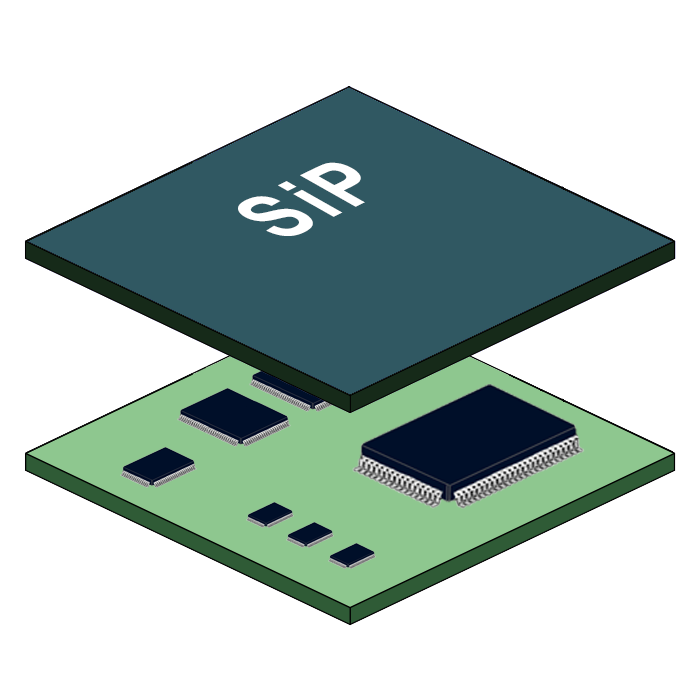
\includegraphics[scale=0.2]{img/System_in_package.png}
  \end{center}
  \fonte{Google Imagens}
  \label{fig:SIP}
\end{figure}
%\Floatbarrier

%%%%%%%%%%%%%%%%%%%%%%%%%%%%%%%%%%%%%%%%%%%%%%%%%%%%%%%%%%%%%%%%%%%%%%
\subsection{Kit de desenvolvimento}
%%%%%%%%%%%%%%%%%%%%%%%%%%%%%%%%%%%%%%%%%%%%%%%%%%%%%%%%%%%%%%%%%%%%%%
Para testar uma solução integrada, pode-se utilizar módulos de desenvolvimento já preparados com o microcontrolador, interface de comunicação serial e sistema de alimentação já dispostos em uma placa de circuito. Estas placas aceleram o desenvolvimento, visto que já estão preparadas para aplicações generalistas. Um ponto negativo pode ser a utilização de espaço desnecessário, visto que elas não são dedicadas para uma aplicação apenas. Entretanto, elas servem de forma apropriada para testes e validação de soluções iniciais antes da confecção de um circuito final.
%%%%%%%%%%%%%%%%%%%%%%%%%%%%%%%%%%%%%%%%%%%%%%%%%%%%%%%%%%%%%%%%%%%%%%
\subsection{Esquema elétrico}
%%%%%%%%%%%%%%%%%%%%%%%%%%%%%%%%%%%%%%%%%%%%%%%%%%%%%%%%%%%%%%%%%%%%%%
Para elaborar todo desenvolvimento eletrônico, utilizou-se a ferramenta Altium\citeonline{Altium2008} que possibilita um sincronismo entre o desenho esquemático e o desenho da placa de circuito impresso. Uma vez que se tenha o desenho da placa de circuito impresso, uma gama de opções se abre para a produção desta placa tanto no mercado nacional como internacional. Devido a um vínculo preestabelecido em outros projetos, utilizou a opção de fabricação na China para obter uma produção rápida e barata, visto que a alta demanda em fabricantes nacionais elevou o tempo de entrega e os custos de produção.
%%%%%%%%%%%%%%%%%%%%%%%%%%%%%%%%%%%%%%%%%%%%%%%%%%%%%%%%%%%%%%%%%%%%%%
\section{\textit{Software}}
%%%%%%%%%%%%%%%%%%%%%%%%%%%%%%%%%%%%%%%%%%%%%%%%%%%%%%%%%%%%%%%%%%%%%%
Para o desenvolvimento da solução de software, cada fabricante possui uma plataforma de desenvolvimento recomendada, bem como compiladores específicos e dedicados para seus produtos. O fabricante ST Microeletronics disponibiliza gratuitamente a ferramenta STM Cube IDE \citeonline{cubeide2022} para desenvolvimento com seus microcontroladores.
Além disso, se faz necessária uma adaptação do software de exemplo fornecido pelo fabricante do microcontrolador escolhido para conversar com o RTC. 
%%%%%%%%%%%%%%%%%%%%%%%%%%%%%%%%%%%%%%%%%%%%%%%%%%%%%%%%%%%%%%%%%%%%%%
\section{Desempenho energético}
%%%%%%%%%%%%%%%%%%%%%%%%%%%%%%%%%%%%%%%%%%%%%%%%%%%%%%%%%%%%%%%%%%%%%%
Para análise do desempenho energético do sistema, se faz necessário o uso de ferramentas como osciloscópio para traçar curvas de carga e a corrente de consumo em cada processo em execução. Entretanto, algumas dessas correntes podem necessitar usar valores disponibilizados diretamente pelos fabricantes dos dispositivos, visto que possuem um consumo extremamente baixo, sendo necessário equipamentos dedicados para esse processo. Entre as ferramentas utilizadas, um destaque especial para o osciloscópio com a captura de pontos para arquivos no formato CSV (\textit{"Comma Separated Values"}, Valores Separados por Vírgula). Estes arquivos podem ser manipulados com a ferramenta Python para transformar um valor de tensão lido em um resistor de \textit{"Shunt"} para a potência de consumo fazendo o uso de outras variáveis do sistema. Além do multímetro para medições diretas.

%%%%%%%%%%%%%%%%%%%%%%%%%%%%%%%%%%%%%%%%%%%%%%%%%%%%%%%%%%%%%%%%%%%%%%